\documentclass[12pt,a4paper]{article}
\usepackage[utf8]{inputenc}
\usepackage[margin=0.8in]{geometry}
\usepackage{graphicx}
\usepackage{booktabs}
\usepackage{hyperref}
\usepackage{caption}
\usepackage{subcaption}
\usepackage{float}
\usepackage{xcolor}

\definecolor{iiitblue}{HTML}{123C85}

\begin{document}

\begin{titlepage}
    \centering
    \vspace*{0.2in}
    
    % Logo
    
\includegraphics[width=0.22\textwidth]{screenshots/iiitk_logo.png} \\
    \vspace{0.15in}
    
    % Institution Details
    {\large\bfseries\color{iiitblue} INDIAN INSTITUTE OF INFORMATION TECHNOLOGY\\ DESIGN AND MANUFACTURING, KURNOOL} \\
    \vspace{0.05in}
    {\small Department of Computer Science and Engineering} \\
    \vspace{0.5in}
    
    % Project Title Header
    {\large\bfseries B.TECH FINAL YEAR PROJECT PROGRESS REPORT} \\
    \vspace{0.3in}
    
    % Project Name
    {\Huge\bfseries\color{iiitblue} EMS-JAFAR} \\
    \vspace{0.15in}
    {\large\itshape Efficient Multi-Scale Feature Upsampling Framework for Dense Vision Tasks} \\
    \vspace{0.3in}
    
    {\color{iiitblue}\rule{\linewidth}{1.5pt}} \\
    \vspace{0.2in}
    
    % Submission Details
    {\large\bfseries\color{iiitblue} Submitted By} \\
    \vspace{0.1in}
    {\large Yashdeep (123CS0077) \\ Rudra Raj (123AD0008)} \\
    \vspace{0.2in}
    {\color{iiitblue}\rule{\linewidth}{1.5pt}} \\
    \vspace{0.3in}
    
    % Guide Details
    {\large\bfseries\color{iiitblue} Project Guide} \\
    \vspace{0.1in}
    {\large Dr. Srinivas Naik} \\
    
    \vfill
    
    % Academic Year
    {\large\bfseries\color{iiitblue} Academic Year 2026--27}
\end{titlepage}

\newpage

\section{Overview of Current Progress}
This progress report summarizes the implementation, benchmarking, and quantitative results of our B.Tech project on dense feature upsampling using the JAFAR framework up to the current phase. All work documented below has been validated on our local machine (RTX 4060 GPU, 8GB VRAM) and is aimed for deployment on the higher memory systems at campus.

\vspace{0.1in}
\noindent The Code is available at: \url{https://github.com/yashdeep-rai/EMS-JAFAR} \\
\noindent (The repository is forked from the original paper and our additions have been merged.)



\section{Quantitative Results (Pascal VOC 2012)}
We evaluated the upsampling performance on the Pascal VOC 2012 validation set (1,449 images) using DINOv2-Small (22M params) and DINOv2-Base (86M params) backbones. The results were obtained by training a 1x1 conv linear probe classifier on top of the upsampled features.

\begin{table}[H]
    \centering
    \caption{Evaluation Summary at $224 \times 224$ Target Resolution.}
    \label{tab:results}
    \begin{tabular}{llcc}
        \toprule
        Backbone Model & Upsampling Method & Pixel Accuracy (\%) & Mean IoU (\%) \\
        \midrule
        \textbf{DINOv2-Small} & Bilinear Baseline & 94.81\% & 79.47\% \\
        \textbf{DINOv2-Small} & \textbf{JAFAR} & \textbf{96.24\%} & \textbf{84.40\%} \\
        \midrule
        \textbf{DINOv2-Base}  & Bilinear Baseline & 93.70\% & 76.40\% \\
        \textbf{DINOv2-Base}  & \textbf{JAFAR} & \textbf{95.83\%} & \textbf{83.13\%} \\
        \bottomrule
    \end{tabular}
\end{table}

\subsection{Backbone Scaling Insights}
\begin{itemize}
    \item \textbf{Consistent Gains}: JAFAR consistently outperforms the standard Bilinear upsampling baseline across both backbone scales.
    \item \textbf{Widening Gap on Larger Models}: As the backbone capacity scales from Small to Base, the Bilinear baseline performance drops from \textbf{79.47\%} to \textbf{76.40\% mIoU} because the wider 768-dimensional features are highly abstract and interpolate poorly. JAFAR successfully decodes this wider channel space, yielding \textbf{83.13\% mIoU} and widening the performance gap over the baseline to \textbf{+6.73\% mIoU} (compared to +4.93\% for the Small backbone).
\end{itemize}

\subsection{DINOv2-Small Validation Screenshots}
\begin{figure}[H]
    \centering
    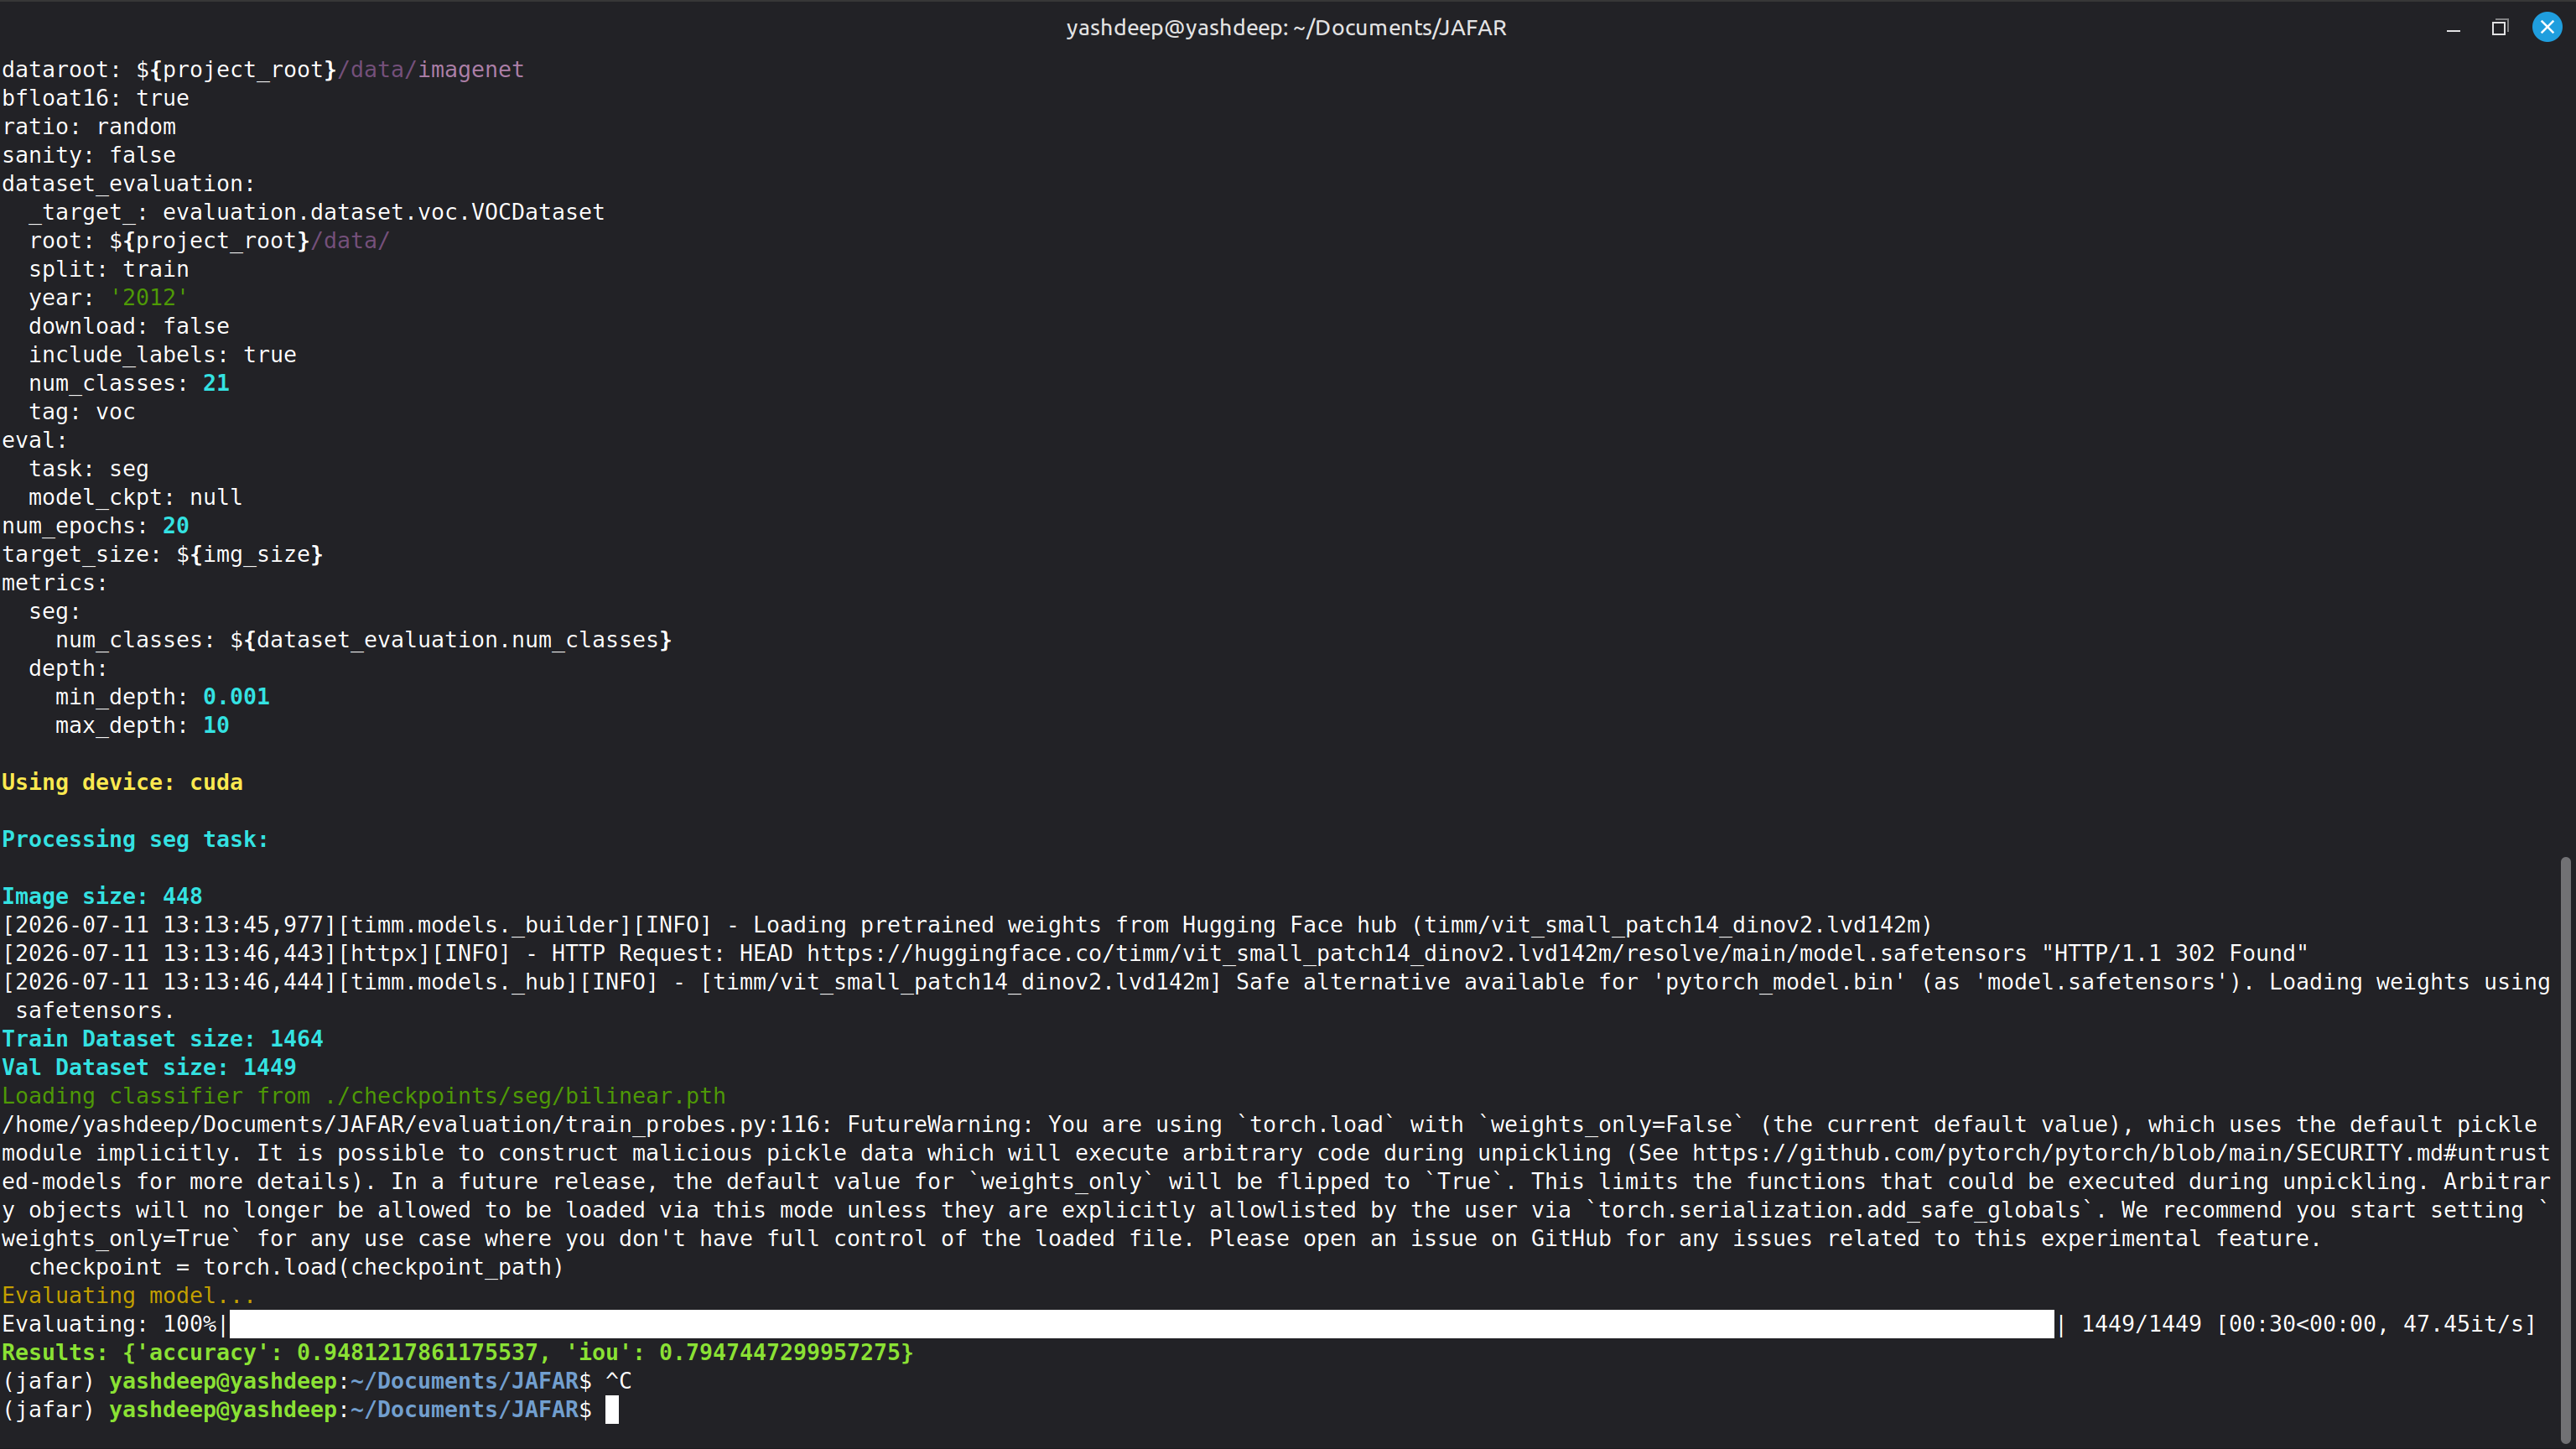
\includegraphics[width=0.85\textwidth]{screenshots/Baseline_Bilinear_part_2.png}
    \caption{Bilinear Validation Run (DINOv2-Small, mIoU: 79.47\%)}
\end{figure}

\begin{figure}[H]
    \centering
    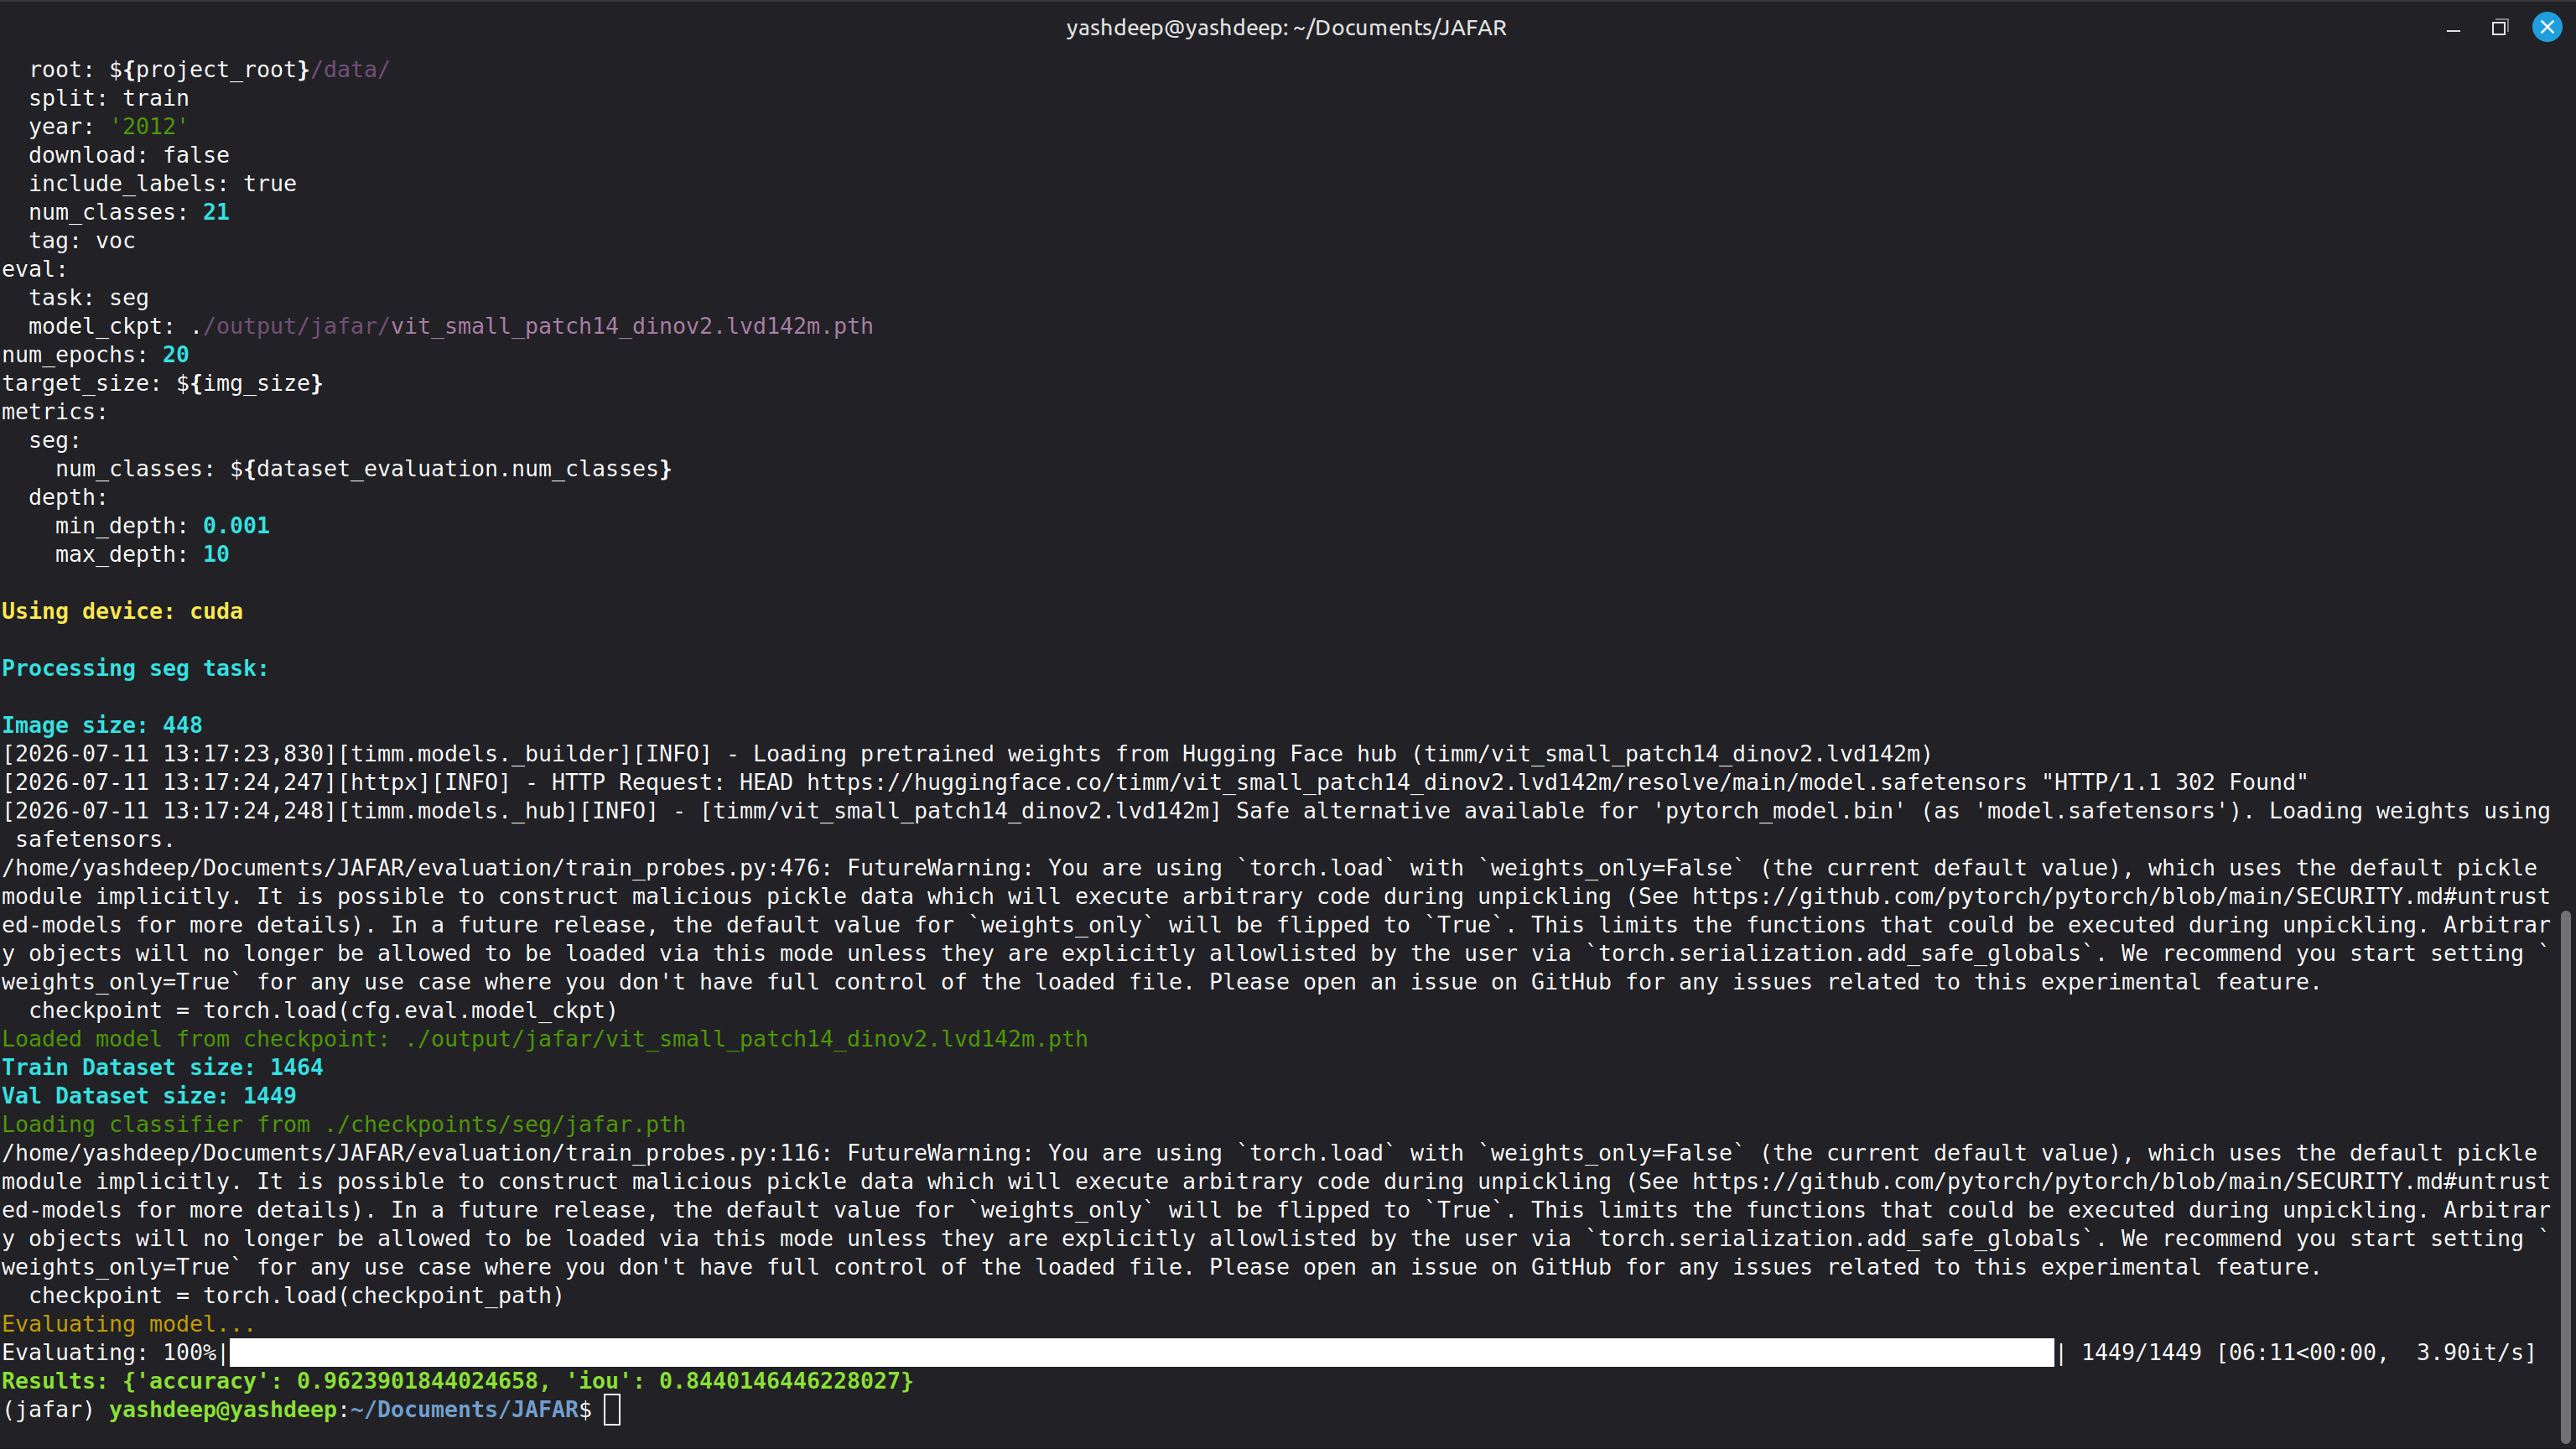
\includegraphics[width=0.85\textwidth]{screenshots/JAFAR_Accuracy_Part_2.png}
    \caption{JAFAR Validation Run (DINOv2-Small, mIoU: 84.40\%)}
\end{figure}

\subsection{DINOv2-Base Validation Screenshots}
\begin{figure}[H]
    \centering
    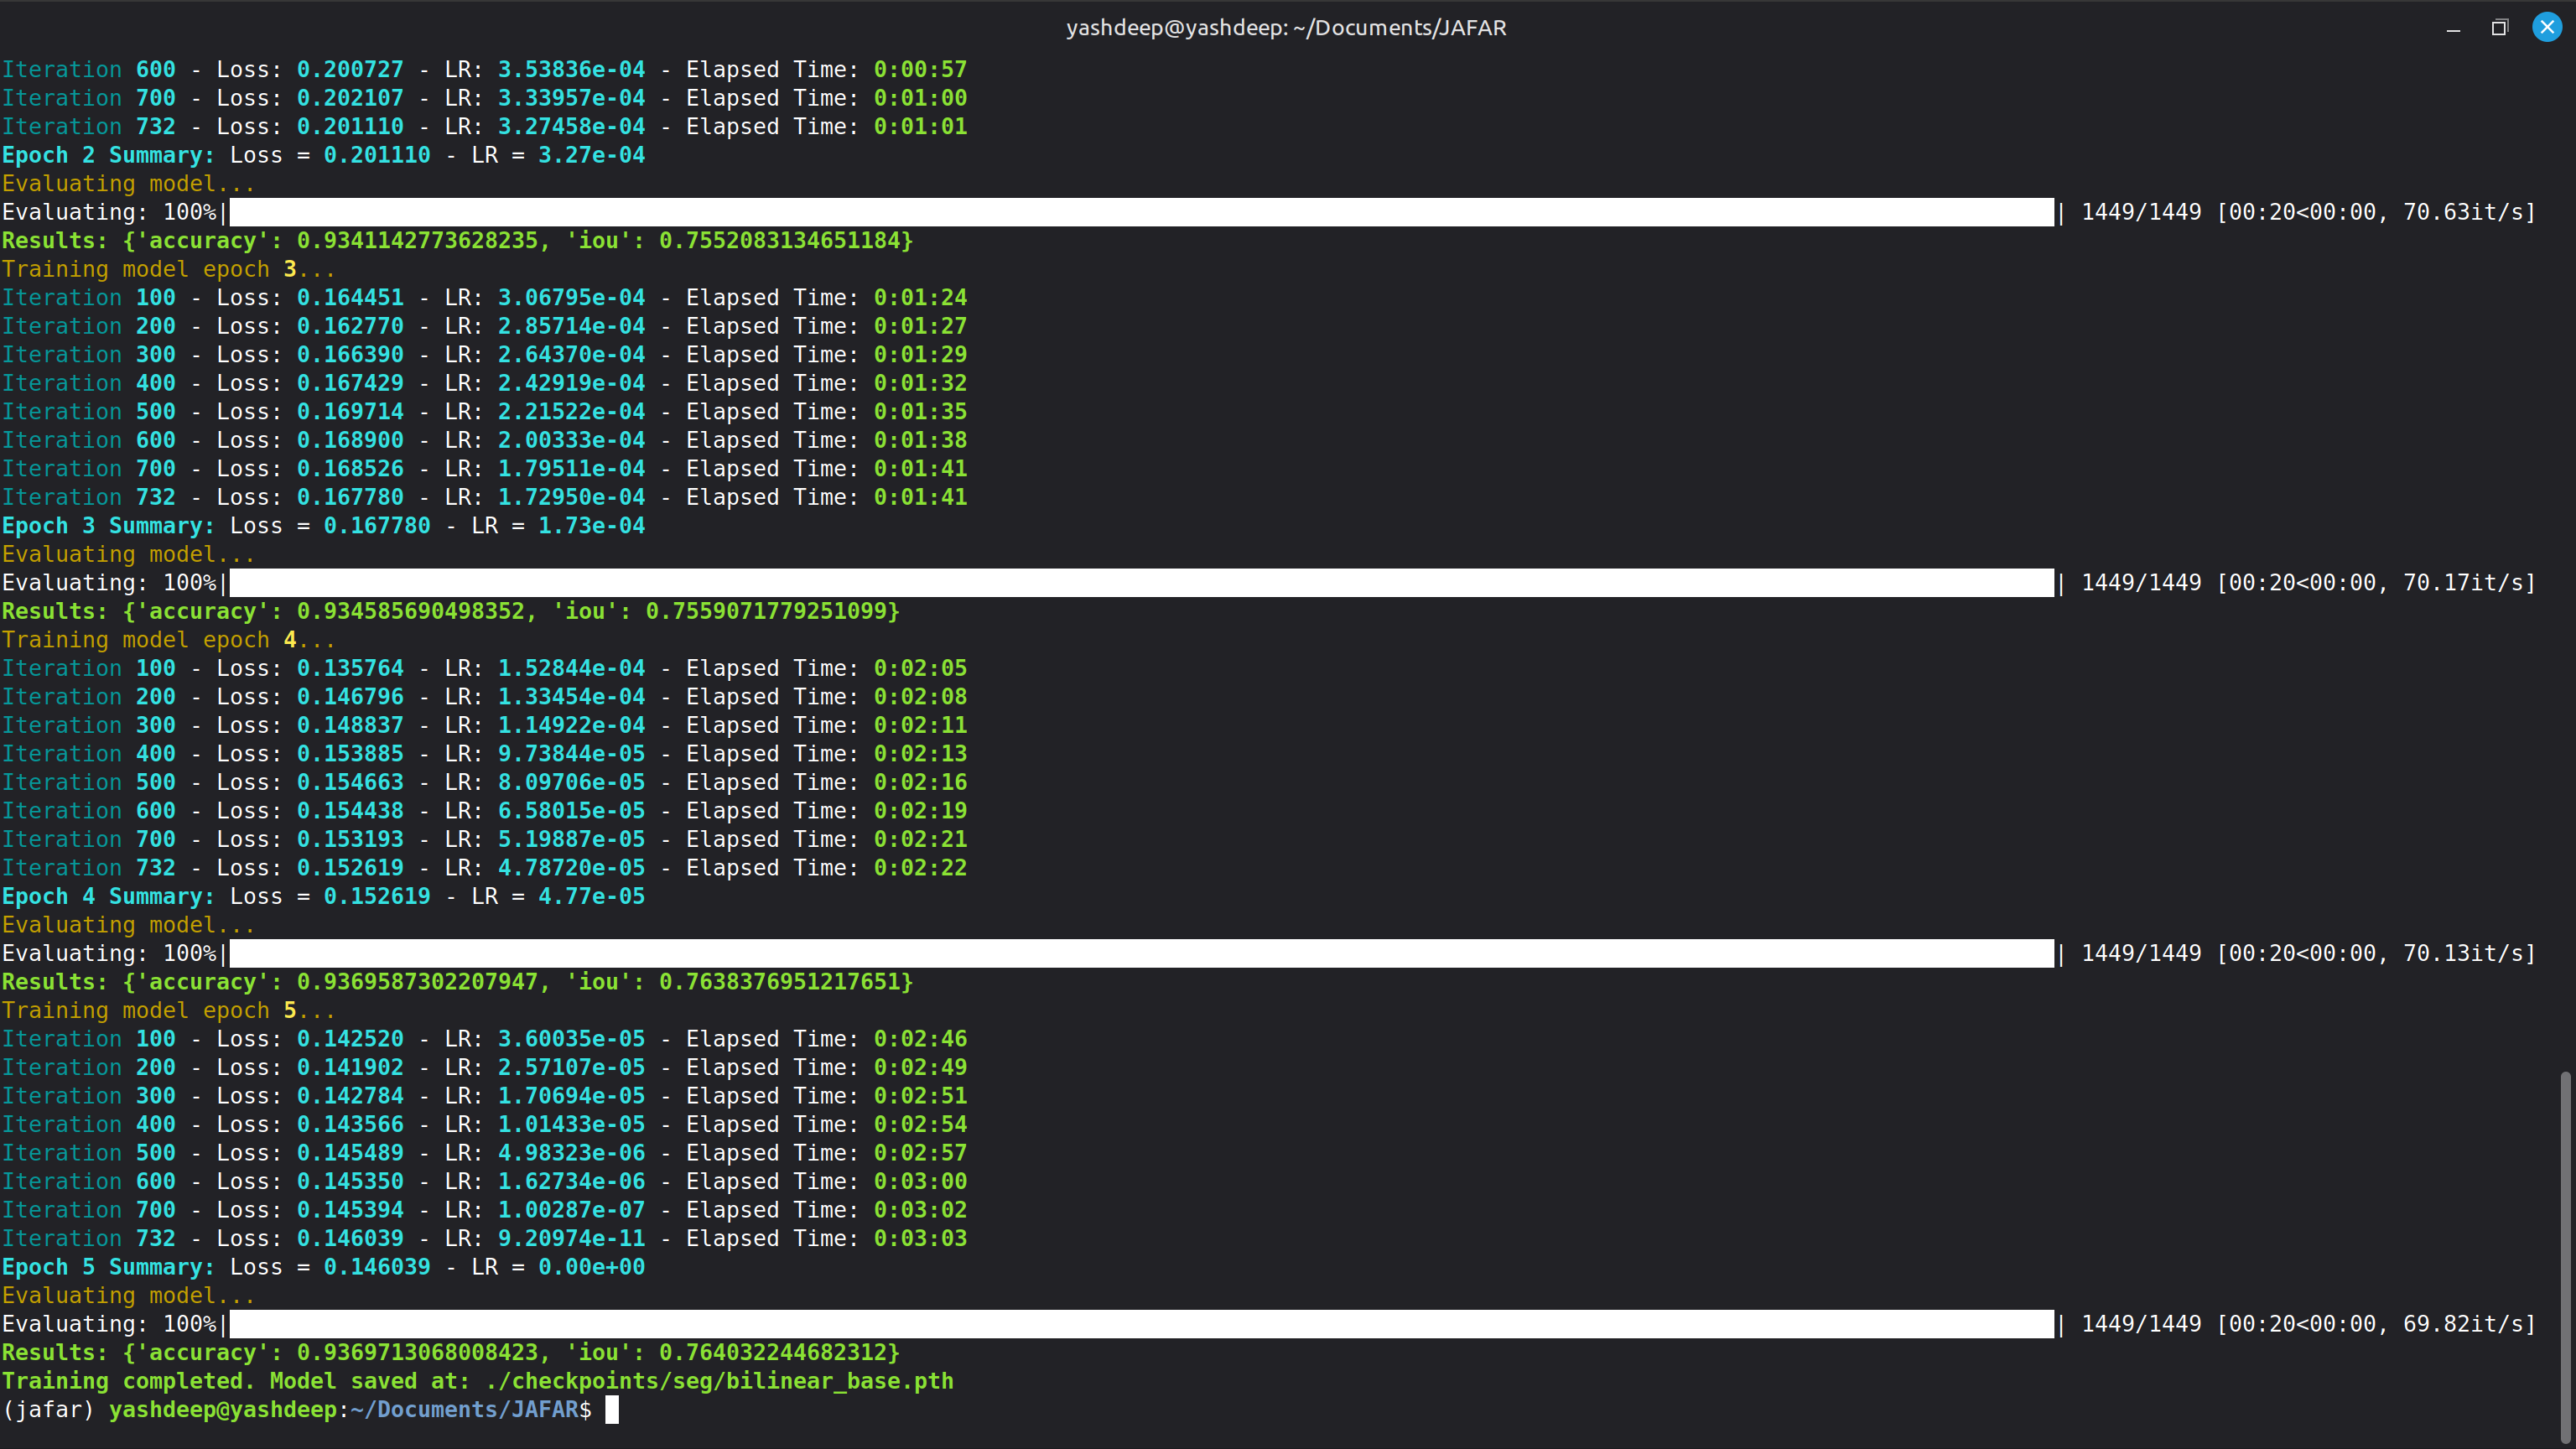
\includegraphics[width=0.85\textwidth]{screenshots/Bilinear_on_Dino_Base.png}
    \caption{Bilinear Validation Run (DINOv2-Base, mIoU: 76.40\%)}
\end{figure}

\begin{figure}[H]
    \centering
    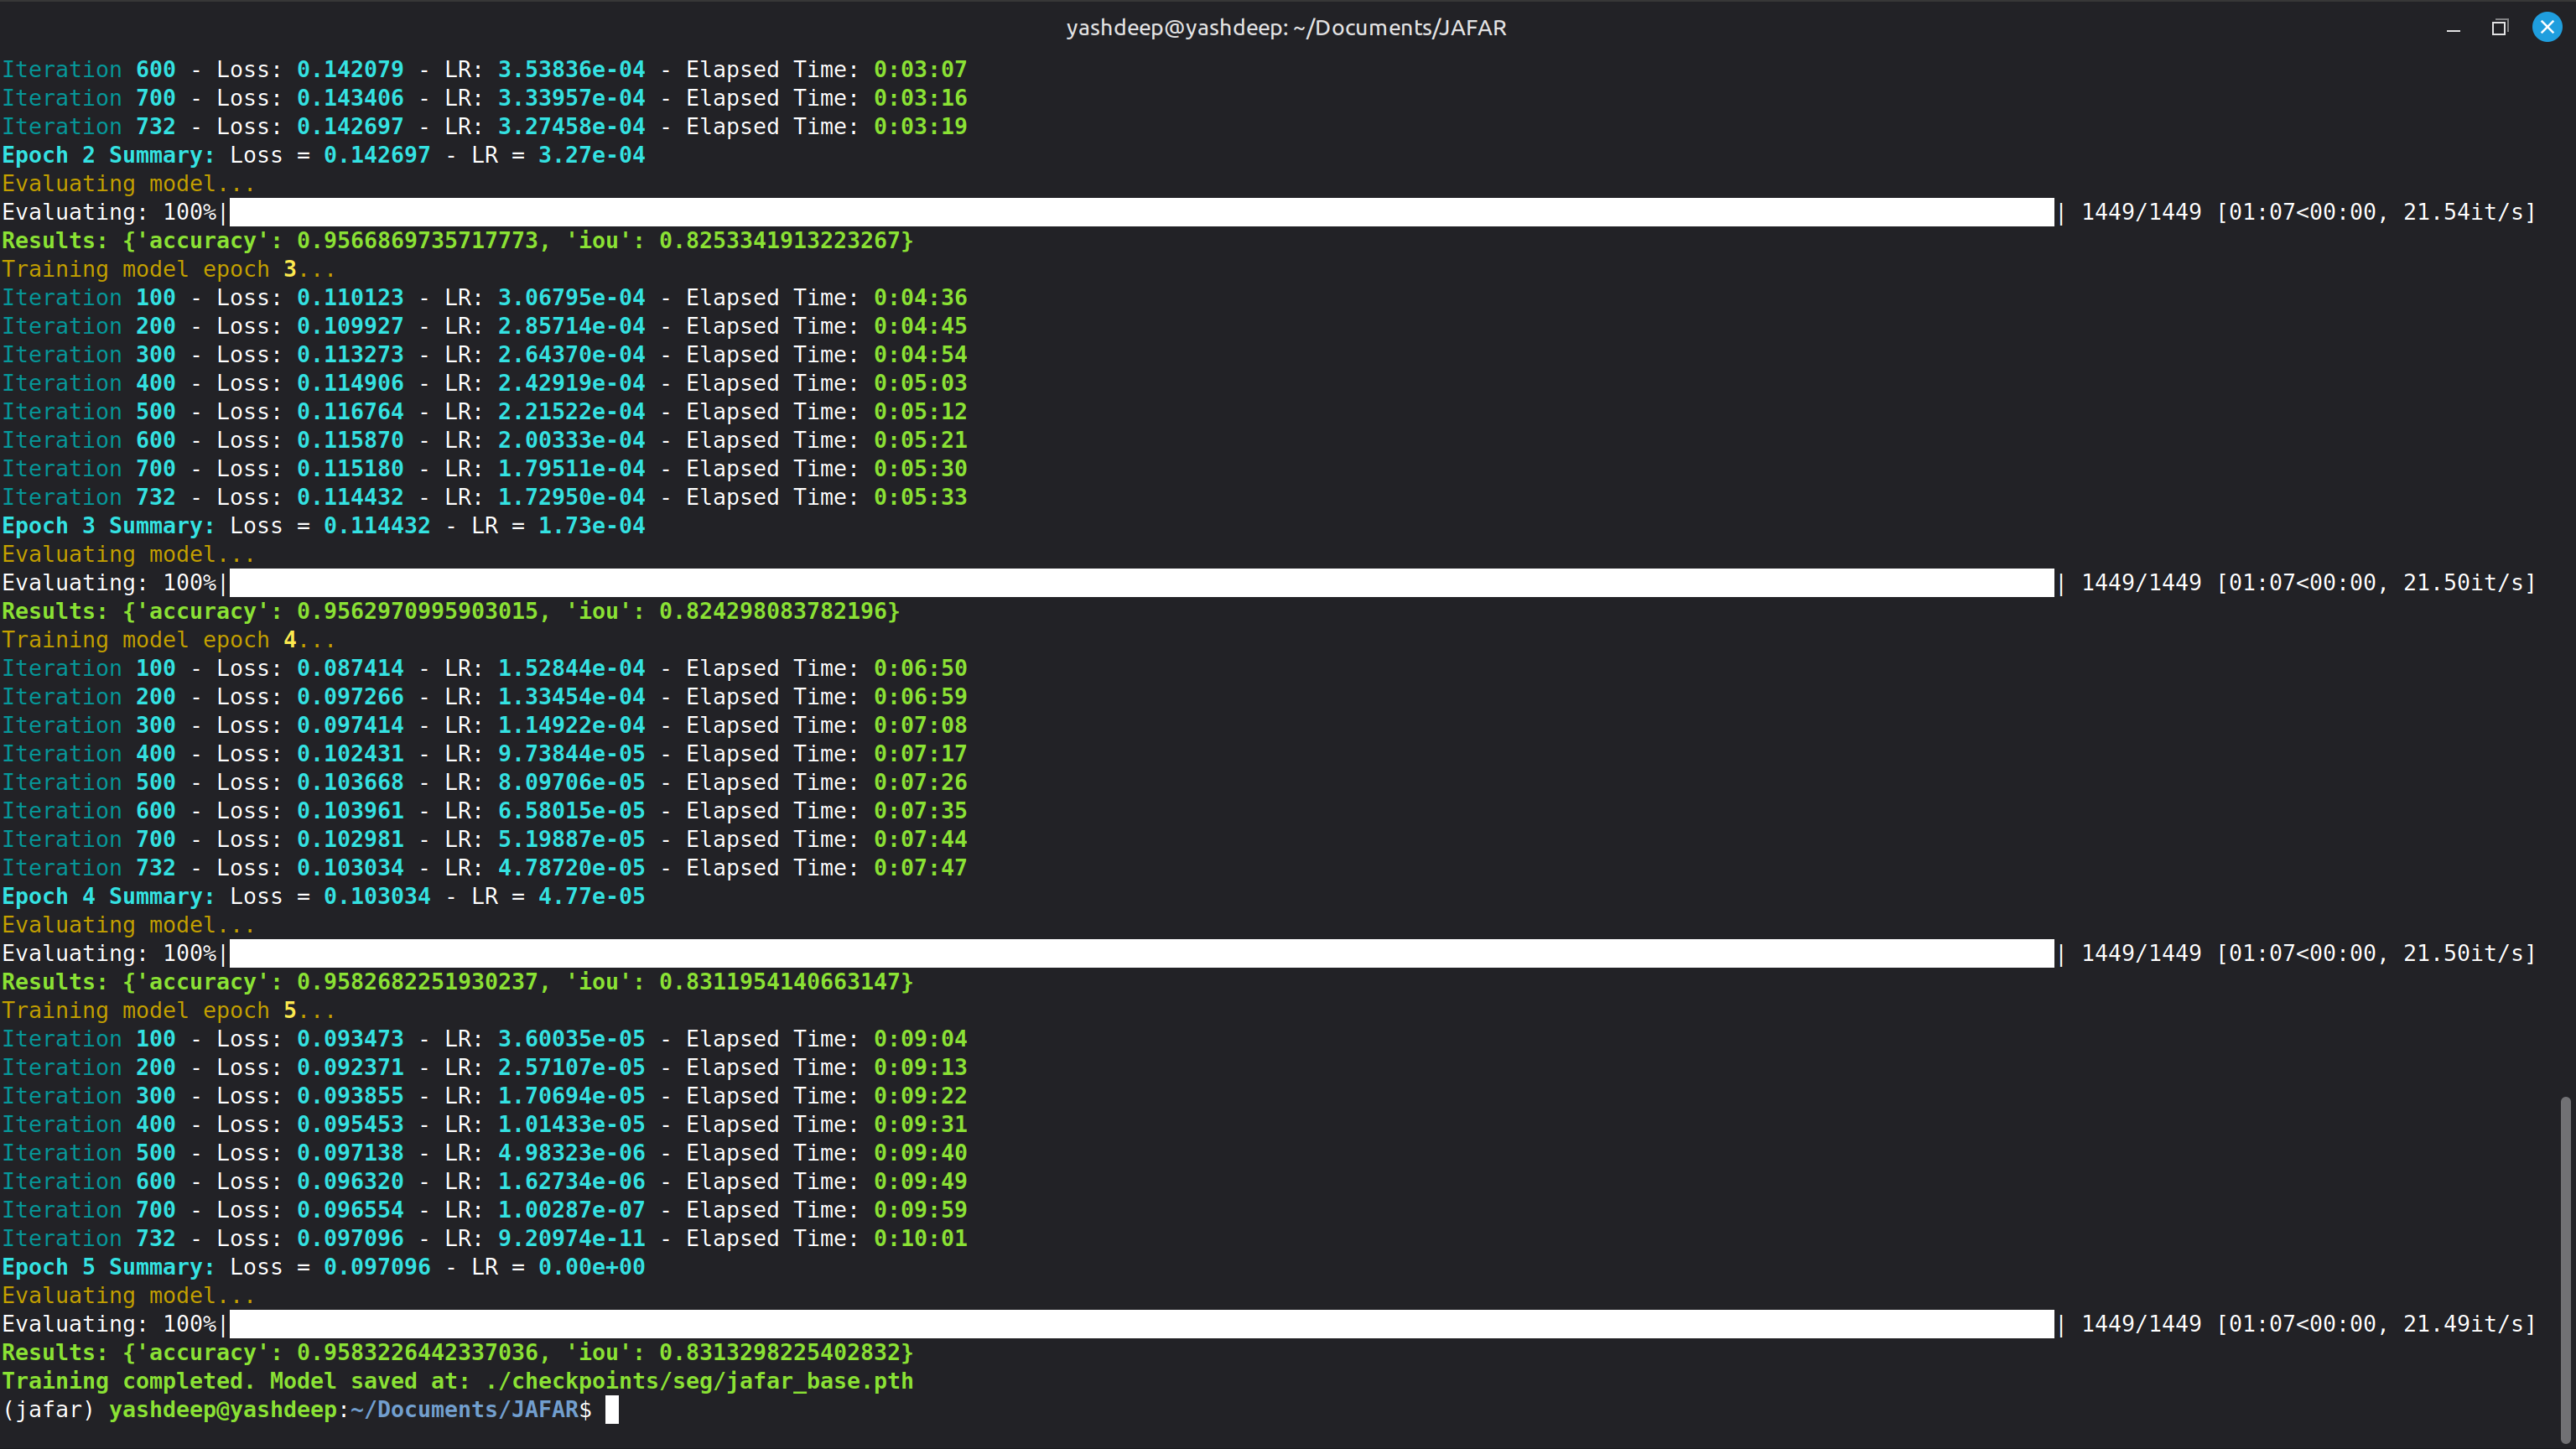
\includegraphics[width=0.85\textwidth]{screenshots/jafar_dino_base.png}
    \caption{JAFAR Validation Run (DINOv2-Base, mIoU: 83.13\%)}
\end{figure}

---

\section{Qualitative Visualizations (PCA Feature Maps)}
The figures below demonstrate the quality of upsampled representations and the final segmentation prediction outputs.

\begin{figure}[H]
    \centering
    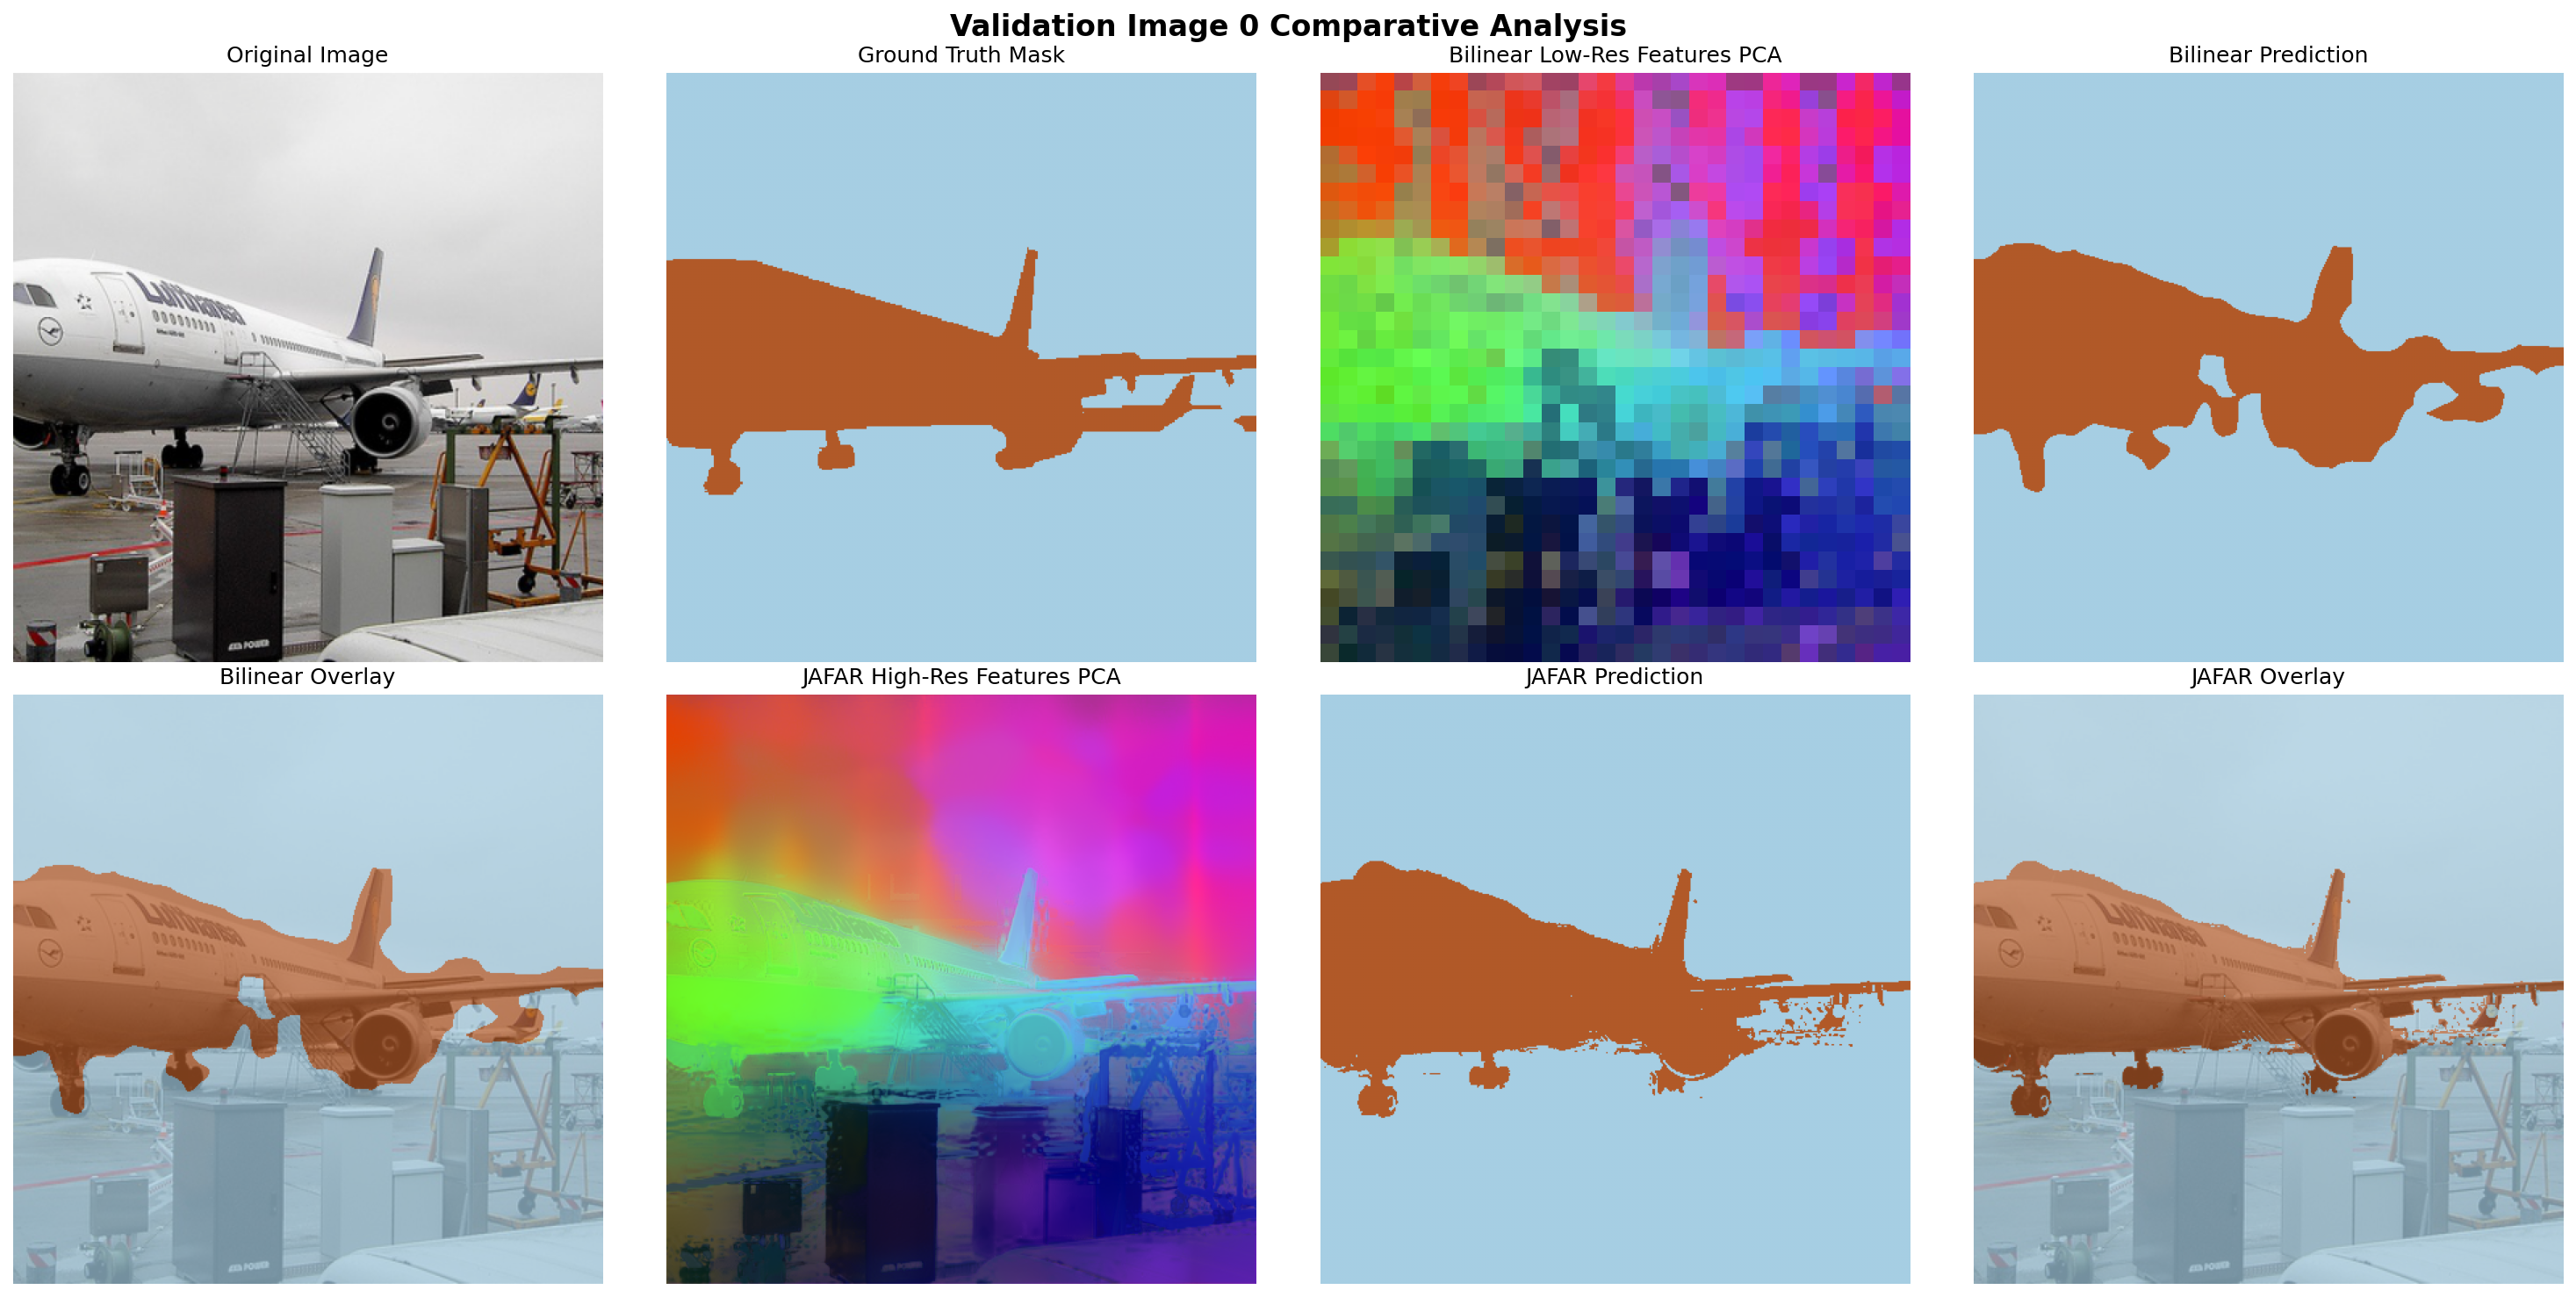
\includegraphics[width=0.9\textwidth]{plots/bilinear_vs_jafar_img_0.png}
    \caption{Comparative prediction and PCA grid showing sharp edge alignment in JAFAR vs. Bilinear.}
\end{figure}

\begin{figure}[H]
    \centering
    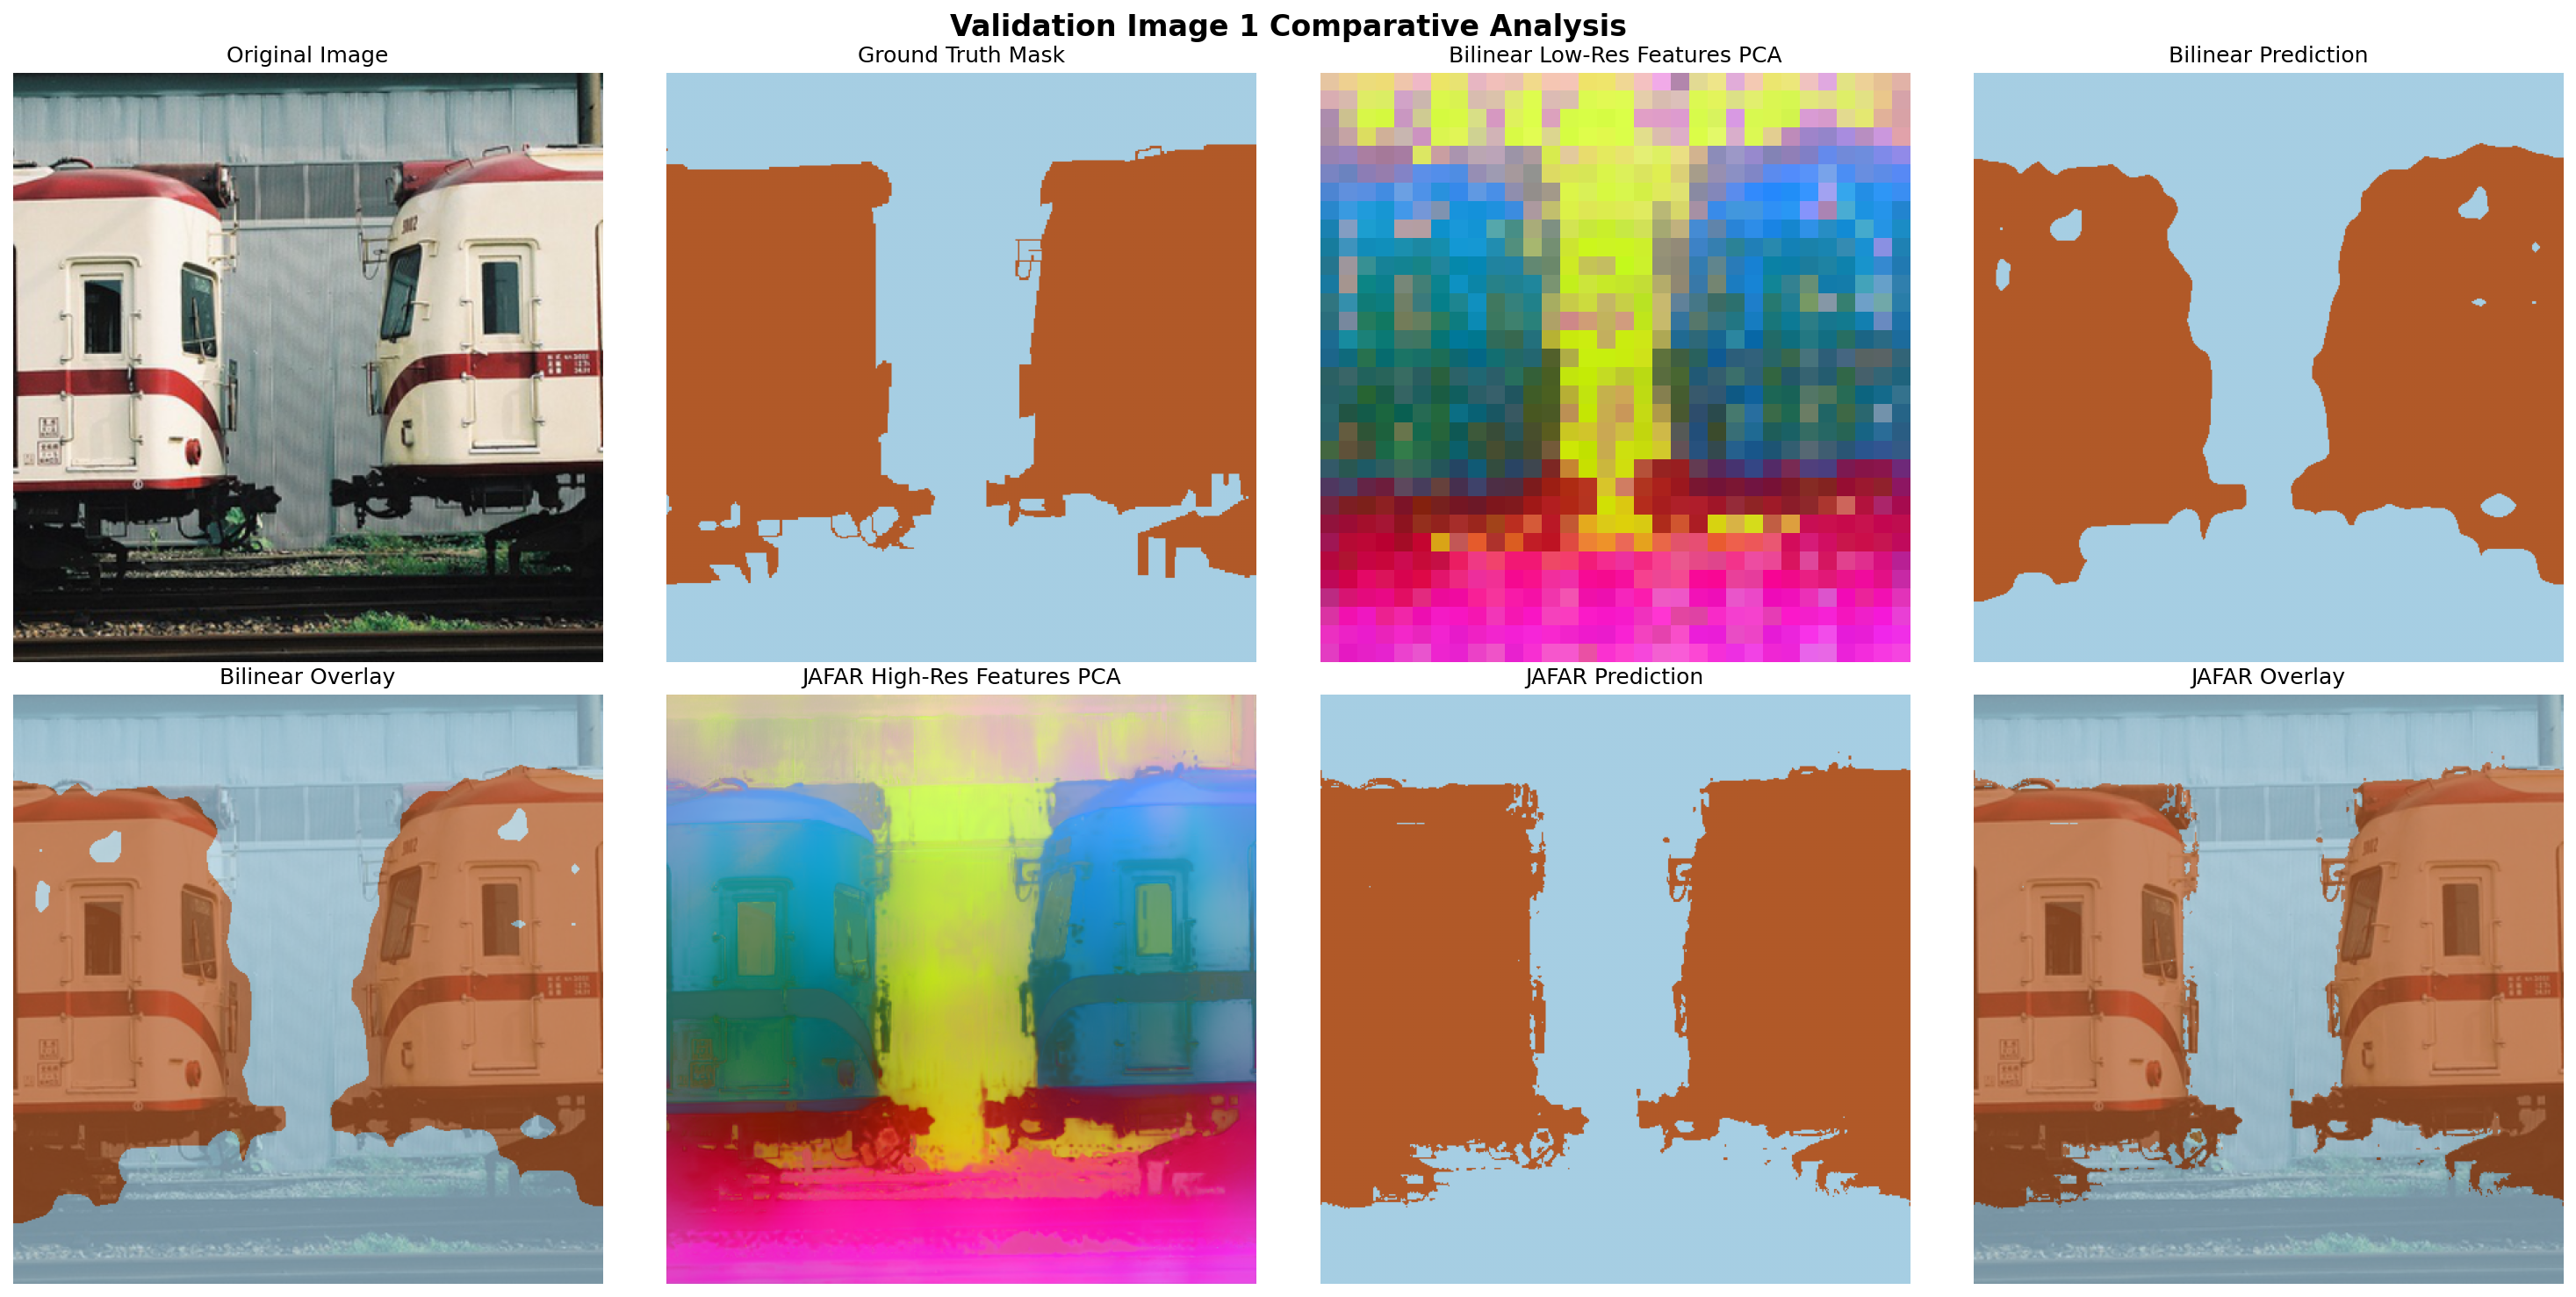
\includegraphics[width=0.9\textwidth]{plots/bilinear_vs_jafar_img_1.png}
    \caption{JAFAR upsampling restores thin structures (like bicycle spokes) that bleed in Bilinear.}
\end{figure}

---

\section{GPU Resource Profiling \& OOM Diagnostics}
Local GPU benchmarks were performed on an \textbf{NVIDIA RTX 4060 Laptop GPU (8GB VRAM)}.

\begin{table}[H]
    \centering
    \caption{Peak GPU memory and compute step times for different resolution scales.}
    \label{tab:profiling}
    \begin{tabular}{lrrrcc}
        \toprule
        Image Size & Forward (ms) & Backward (ms) & Peak VRAM (MB) & Status \\
        \midrule
        56 $\times$ 56   & 6.61 ms  & 21.11 ms & 728.82 MB   & Passed \\
        112 $\times$ 112 & 6.79 ms  & 22.34 ms & 1,092.27 MB & Passed \\
        224 $\times$ 224 & 30.09 ms & 83.76 ms & 3,246.14 MB & Passed \\
        448 $\times$ 448 & 228.22 ms& ---      & $>$ 8,192 MB & Failed (OOM) \\
        \bottomrule
    \end{tabular}
\end{table}

\subsection{Profiling Insights}
\begin{itemize}
    \item \textbf{Attention Memory Bottleneck}: Training JAFAR at $448 \times 448$ resolution is bottlenecked by the $O(N^2)$ memory scaling of the query vectors in the cross-attention layer, triggering a CUDA OOM crash.
    \item \textbf{Multi-Scale Fusion Efficiency}: Fusing 3 layers only adds \textbf{5.44 MB of VRAM overhead} and \textbf{0\% execution time overhead} compared to the 1-layer JAFAR model at $224 \times 224$. This confirms that our proposed $1 \times 1$ Conv Multi-Scale Fusion is computationally efficient.
\end{itemize}

\begin{figure}[H]
    \centering
    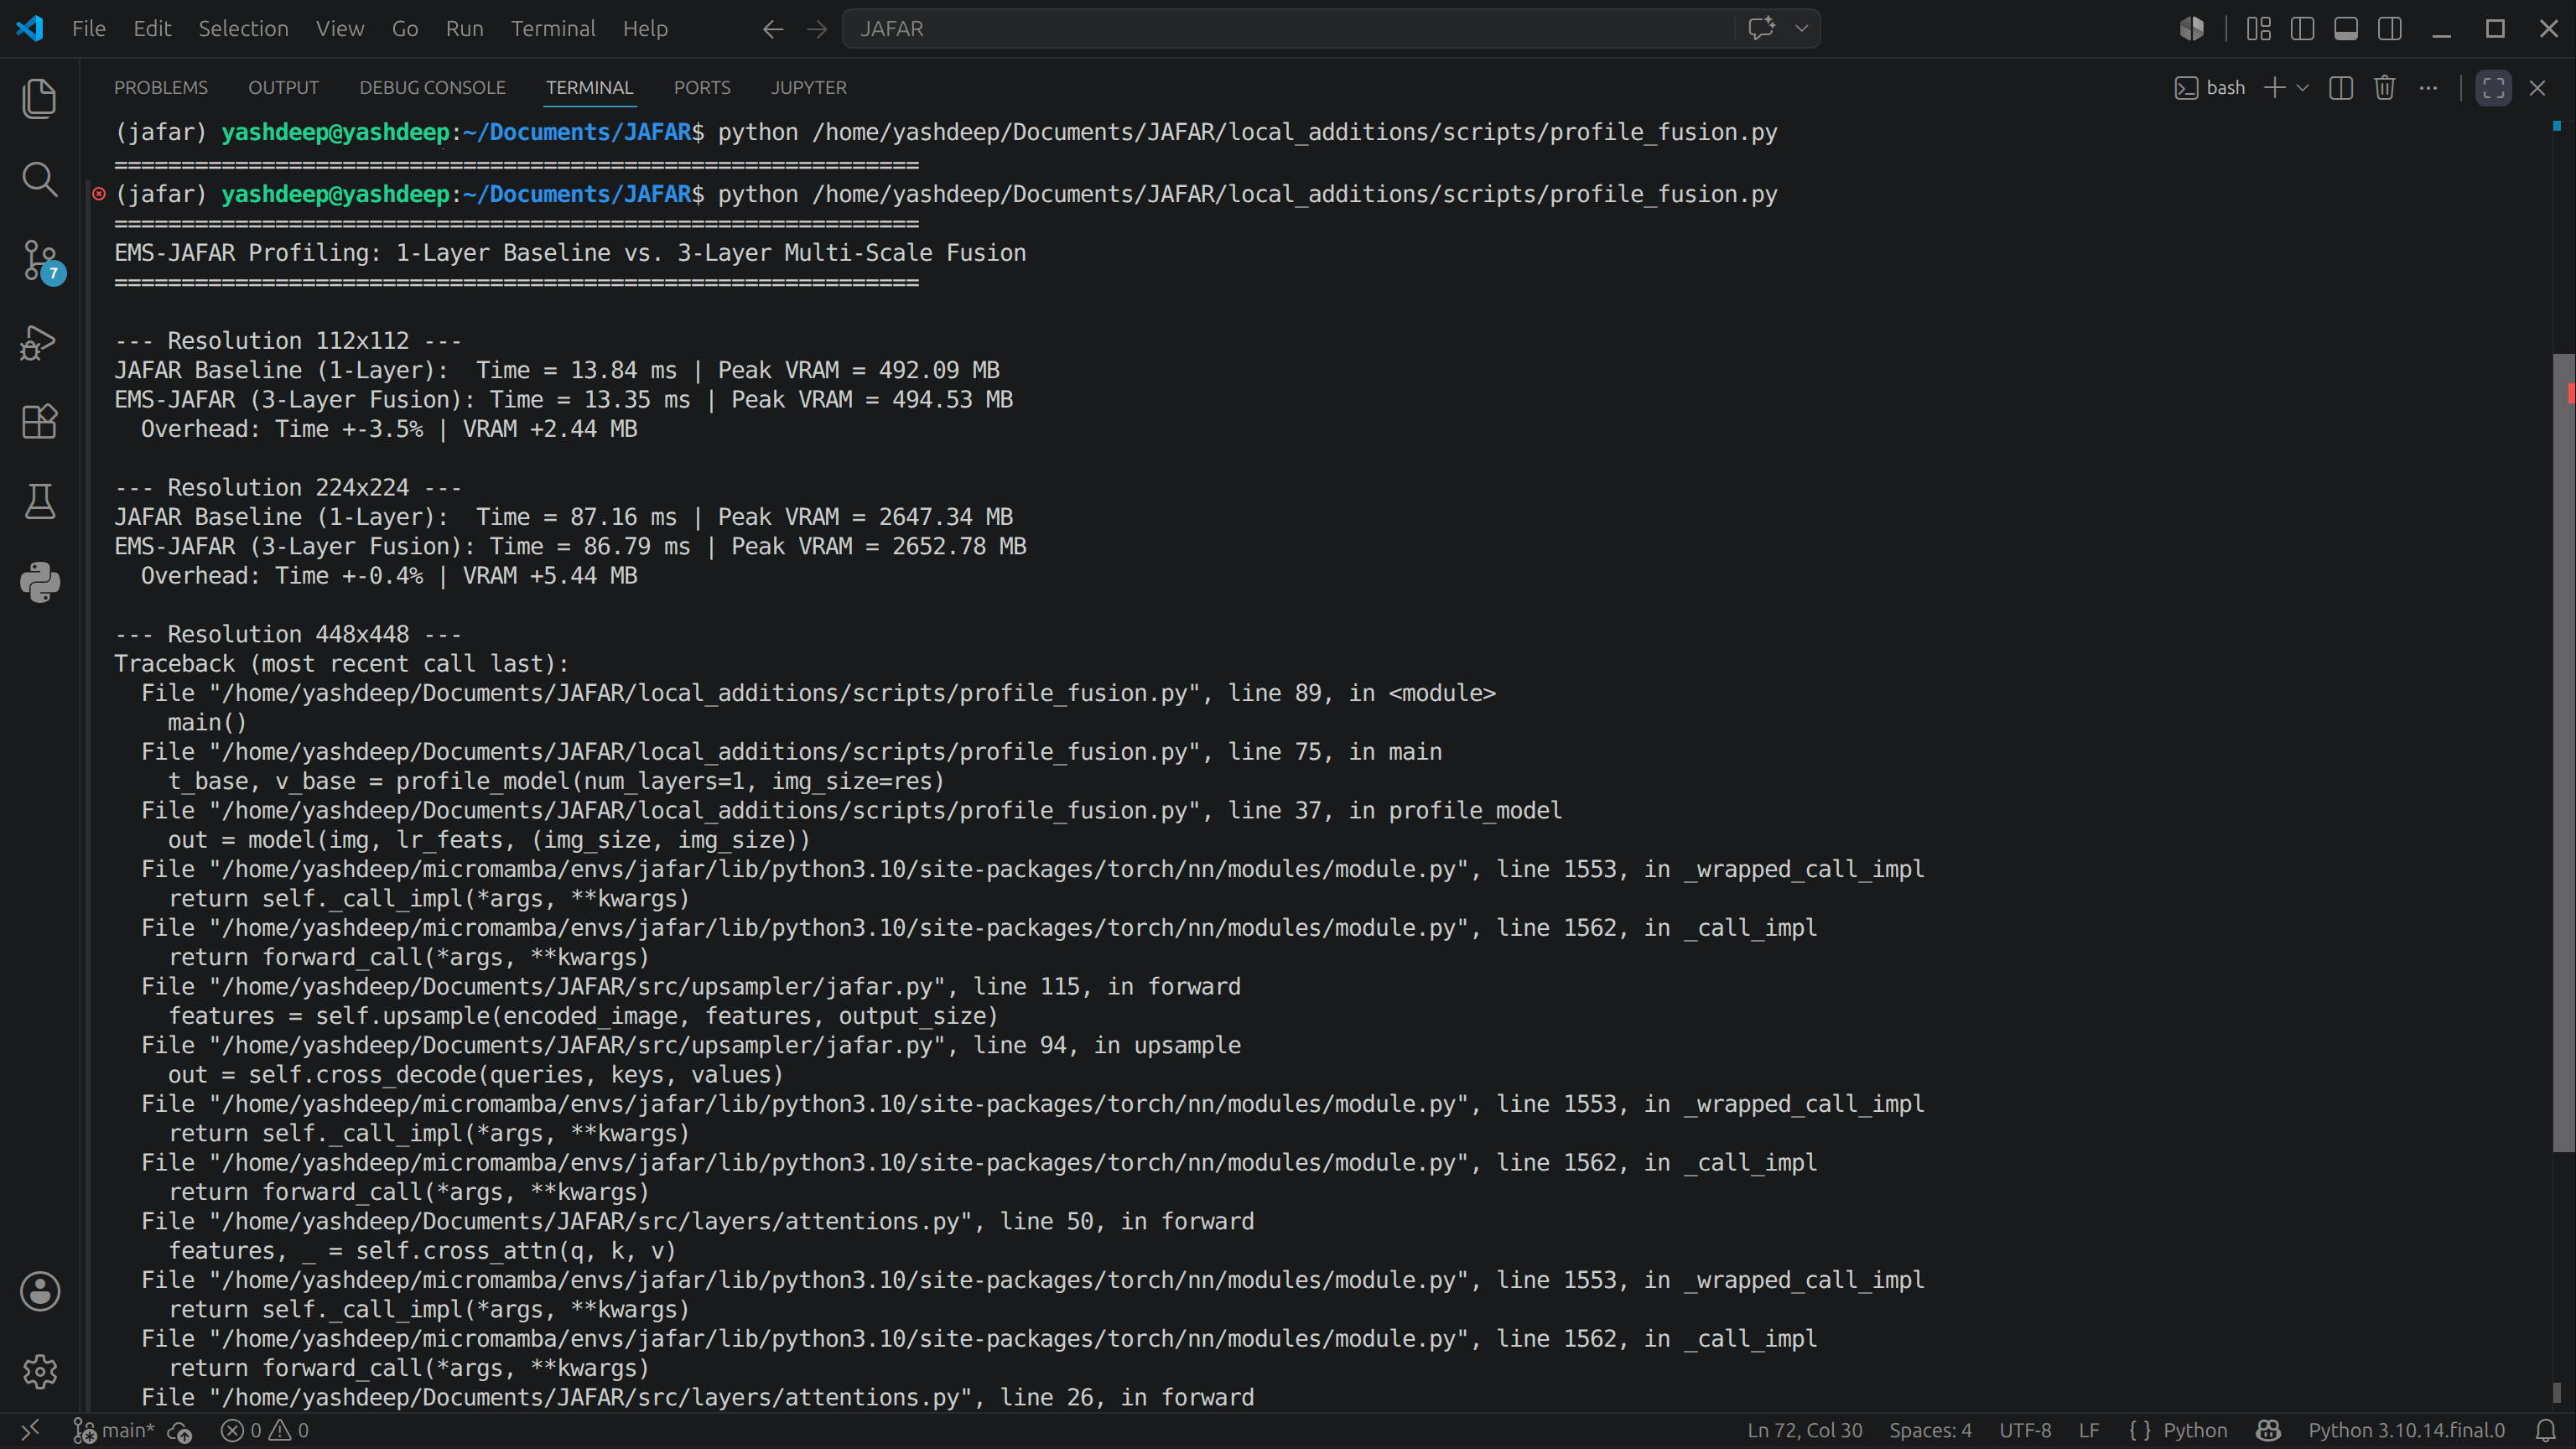
\includegraphics[width=0.75\textwidth]{screenshots/Profile_Fusion_OOM_Error_on_448_448.png}
    \caption{Traceback from local CUDA Out-of-Memory (OOM) error encountered during $448 \times 448$ training.}
\end{figure}

\begin{figure}[H]
    \centering
    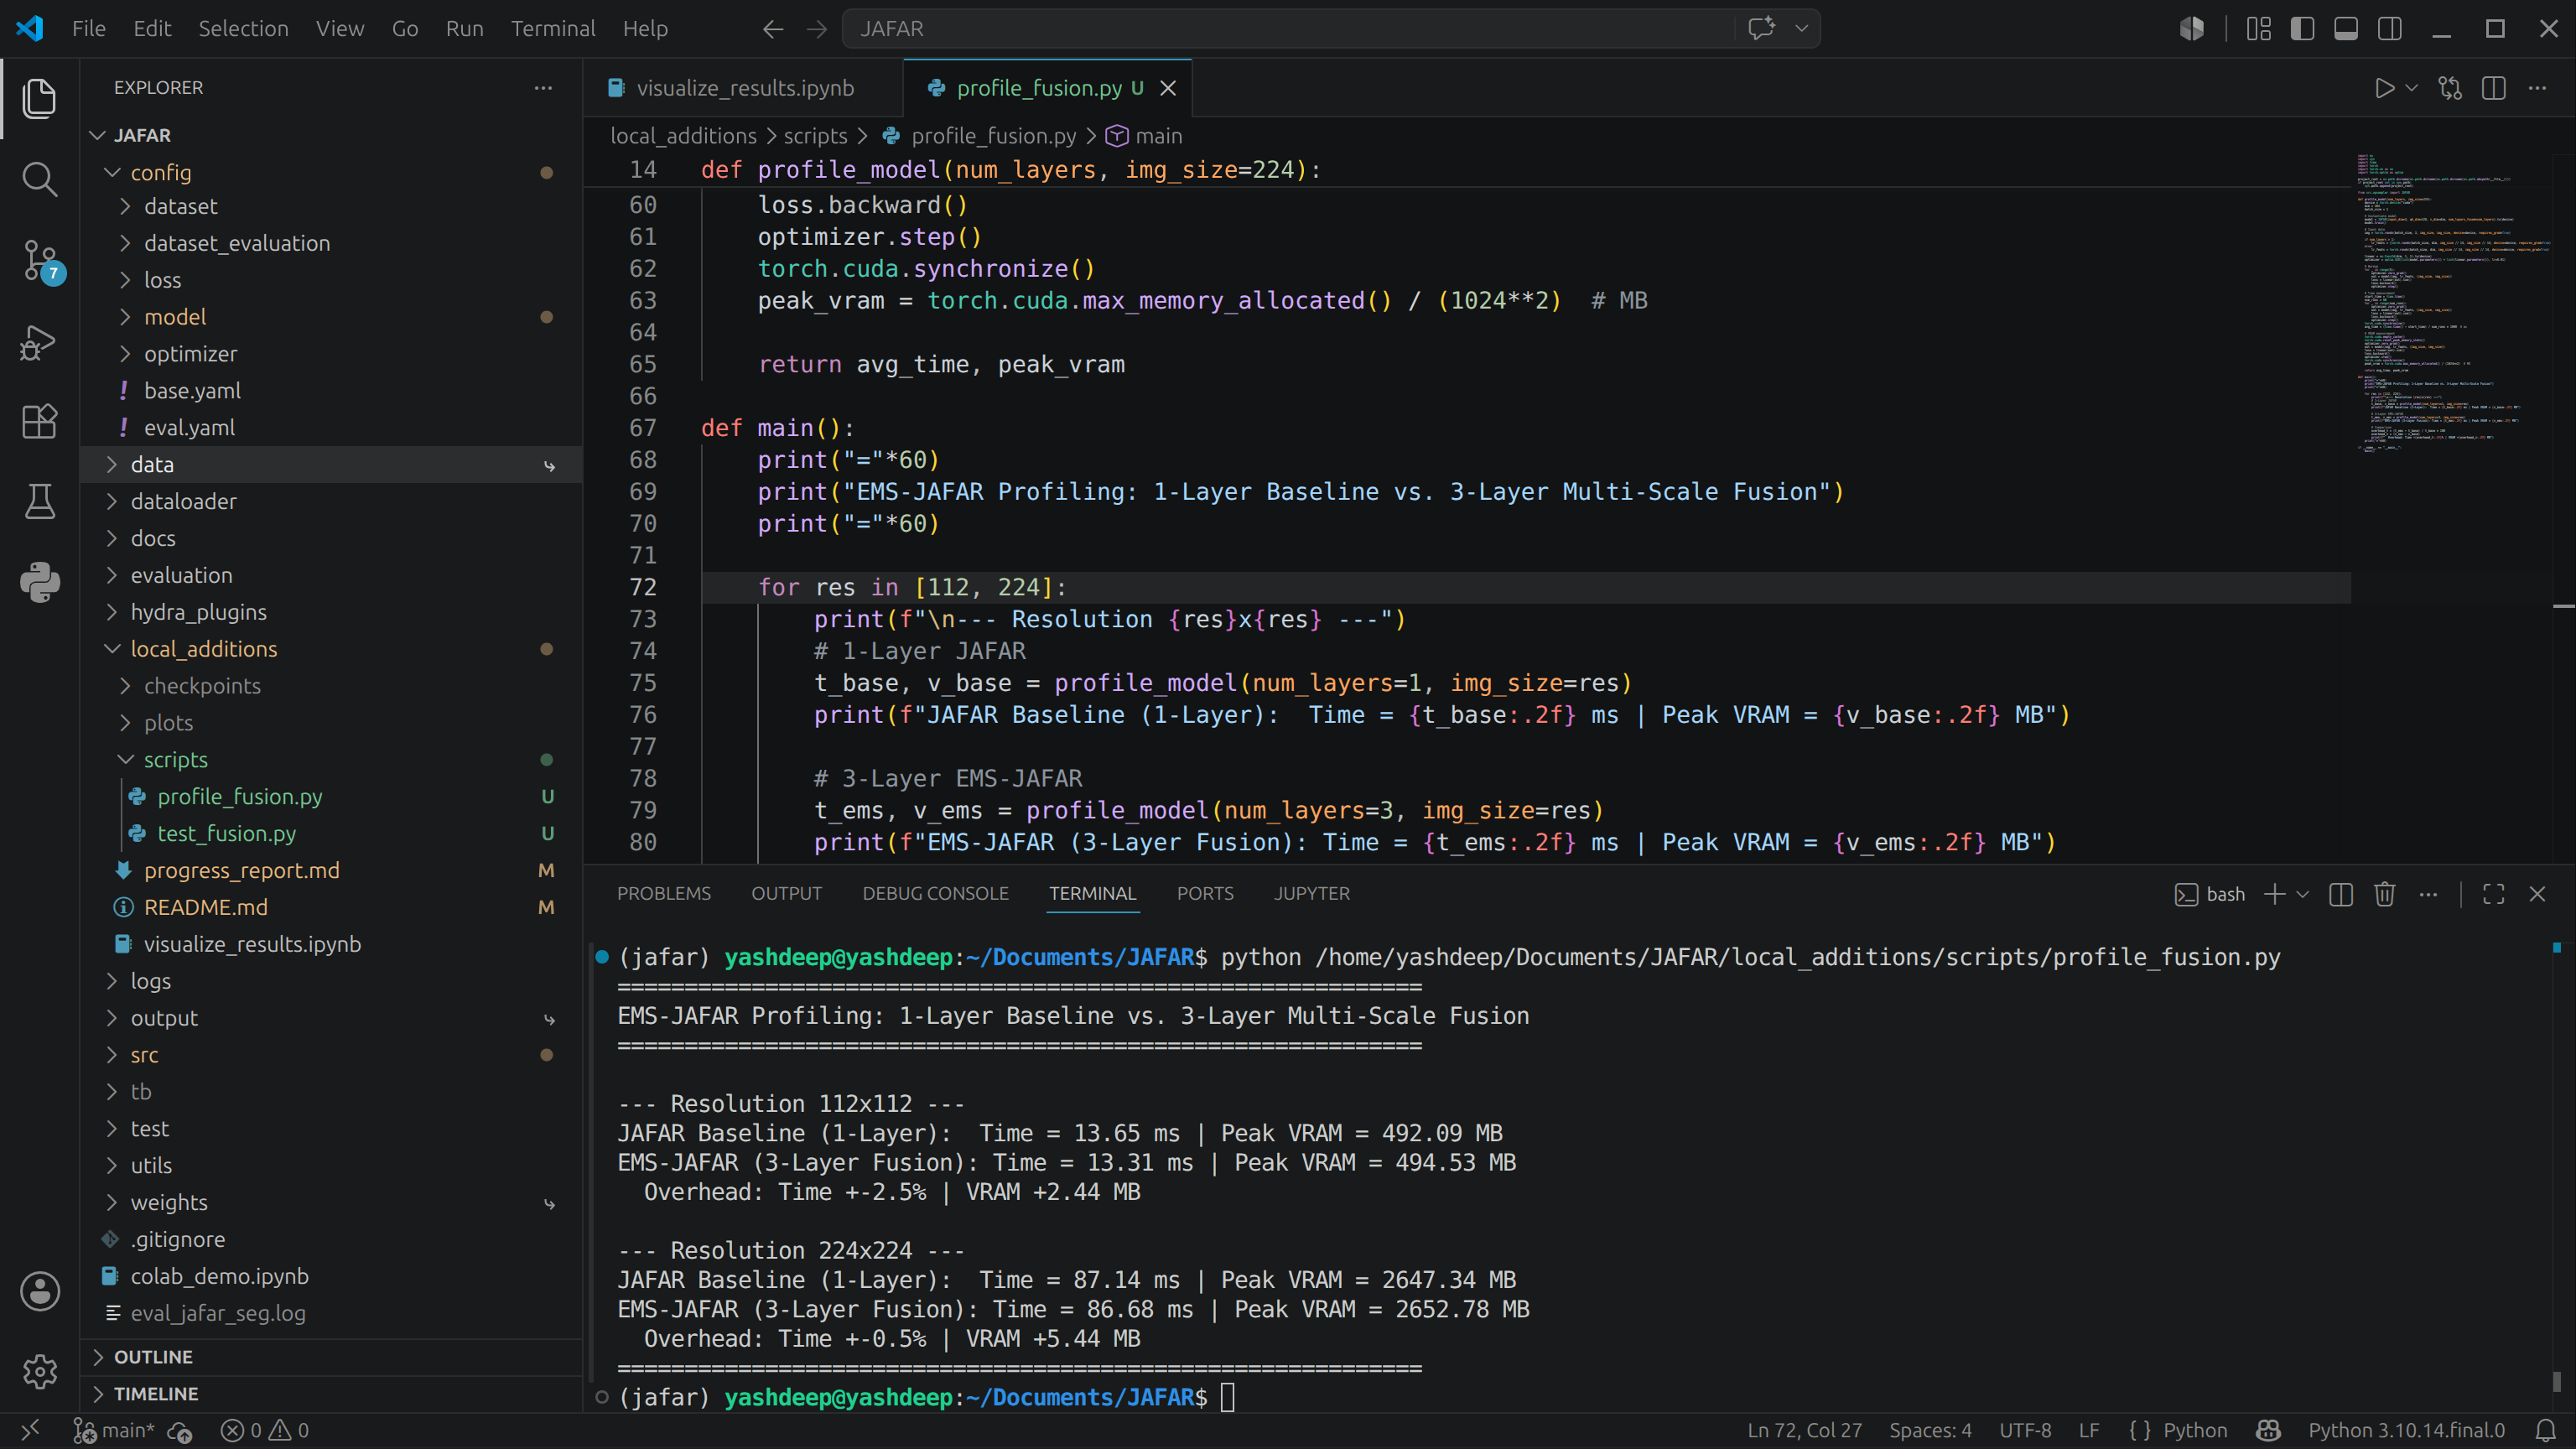
\includegraphics[width=0.75\textwidth]{screenshots/Profile_Fusion_Results.png}
    \caption{Terminal profiling results comparing 1-layer baseline JAFAR with 3-layer EMS-JAFAR.}
\end{figure}

---

\section{Next Steps \& Campus Lab Deployment}
With access to the college lab's high-memory GPU cluster, we are aiming to proceed with:
\begin{enumerate}
    \item \textbf{High-Resolution Training}: Train the JAFAR upsampler model at the target $448 \times 448$ scale to evaluate its full boundary alignment potential.
    \item \textbf{End-to-End EMS-JAFAR Training}: Fine-tune the multi-scale fusion weights on the lab cluster and evaluate the quantitative mIoU gain over the baseline JAFAR model.
    \item \textbf{Depth Estimation}: Train and validate depth estimation probes on the NYU Depth V2 dataset to confirm task-agnostic generalization.
\end{enumerate}

\end{document}
